\section{Theoretischer Hintergrund}
Jedes beliebige \textbf{lineare Netzwerk}, welches aus Widerständen, Spannungs- und Stromquellen, 
Kapazitäten und Induktivitäten besteht, kann durch eine \textbf{Ersatzschaltung} mit einer
Strom- oder Spannungsquelle und einem Widerstand (Impedanz) dargestellt werden. Dabei verhält
sich das Netzwerk von aussen genau gleich wie die entsprechende Ersatzschaltung.
\\\\
Reale Quellen können in gewissen Betriebspunkten durch lineare Netzwerke angenähert (linearisiert) werden. Dieses linearisierte Netzwerk kann sich mit dem Betriebspunkt massiv
ändern.
\\\\
Dieser Versuch hat folgende Zielsetzungen:
\begin{enumerate}[$a)$]
\item Anwenden der \textbf{Norton} und \textbf{Thevenin Ersatzschaltung}
\item Anwenden von \textbf{Strom-} und \textbf{Spannungsfehlerschaltung}
\item Messen und Auswerten von \textbf{Kennlinien}
\item Netzgeräte kennen lernen
\item \textbf{Unterschied} zwischen Strom- und Spannungsquelle lernen
\end{enumerate}
\section{Diskussion}
\section{Theoretische Aufgaben}
\subsection{Batterie}
Nehmen Sie mindestens eine Batterie von sich zu Hause mit, welche Sie im Labor ausmessen
möchten. Diese Batterie werden wir entladen. Sie wird nicht mehr brauchbar sein.
\subsection{Aufgaben}
\begin{enumerate}[$a)$]
\item Von einer Autobatterie werden folgende zwei Punkte gemessen: ($U_1=13.80\text{V}$, $I_1=10.0\text{A}$) und ($U_2=10.20\text{V}$, $I_2=150.0\text{A}$).
Berechnen Sie nun numerisch den Innenwiderstand, die Leerlaufspannung und den
Kurzschlussstrom.
\item Ist die Autobatterie eher eine Strom- oder Spannungsquelle?
\item Skizzieren Sie die Kennlinien von einer idealen Strom- und Spannungsquelle. Wie unterscheiden sie sich von realen Quellen?
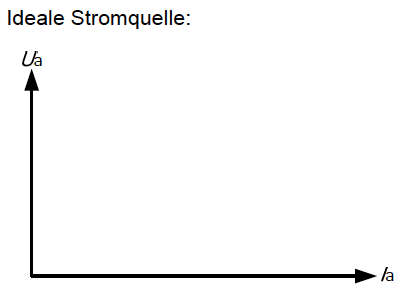
\includegraphics[scale=0.5]{../img/III/IIIa}
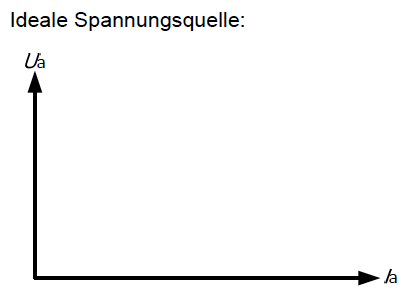
\includegraphics[scale=0.5]{../img/III/IIIb}
\\\\
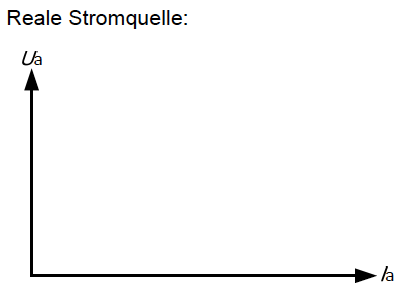
\includegraphics[scale=0.5]{../img/III/IIIc}
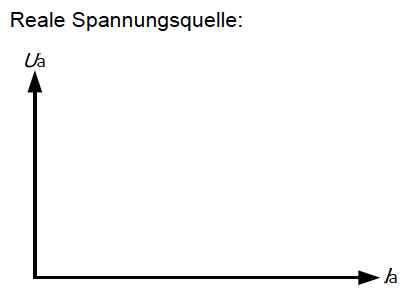
\includegraphics[scale=0.5]{../img/III/IIId}
\end{enumerate}
\section{Versuchsanleitung}
\subsection{Kennlinie eines Labornetzgerätes}
\subsubsection{Messaufgabe}
Messen Sie die $U/I$-Kennlinie des Labornetzgerätes. Stellen Sie die Leerlaufspannung auf $U_N=10.0\text{V}$ ein.
\subsubsection{Messerwartung}
\subsubsection{Messaufbau und Kommentare}
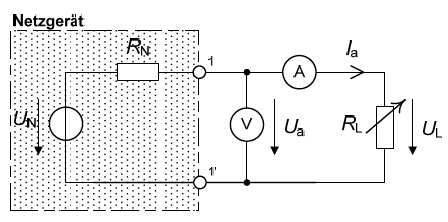
\includegraphics[scale=1]{../img/III/IIIe}
\subsubsection{Messresultate und Berechnungen}
Stellen Sie die Strombegrenzung zuerst auf das Maximum. Zeichnen Sie die Kennlinie in ein Diagramm Ua=f(Ia). Stellen Sie die Strombegrenzung dann auf verschiedene Werte und wiederholen Sie die Messungen. Zeichnen Sie die verschiedenen Kurven in das untenstehende Diagramm, mit dem Begrenzungsstrom als Parameter.\\
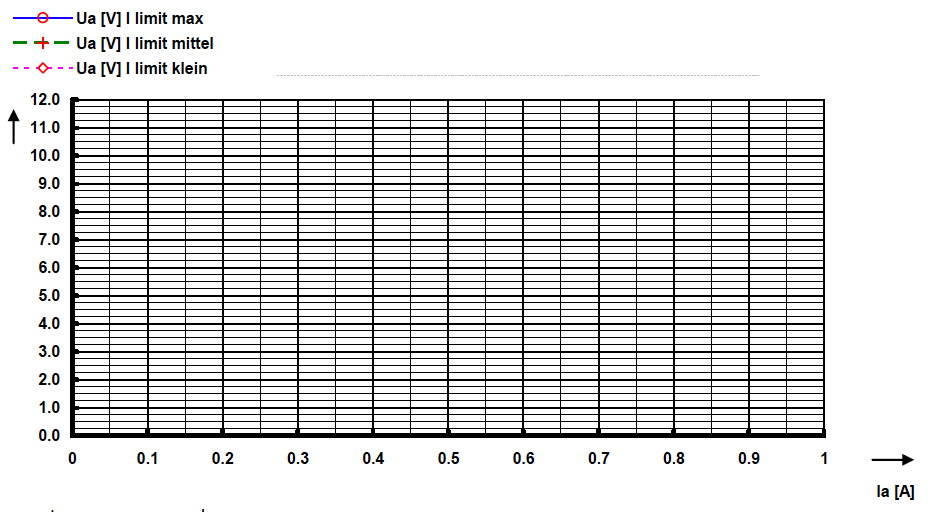
\includegraphics[scale=0.5]{../img/III/IIIf}
\\
\textbf{Messwert:} $I_{\text{limit}}=\text{max}$\\
\begin{tabular}{|c|c|c|c|c|c|c|c|c|c|c|}\hline
$I_a/\text{A}$&&&&&&&&&&\\\hline
$U_a/\text{V}$&&&&&&&&&&\\\hline
\end{tabular}
\\
\textbf{Messwert:} $I_{\text{limit}}=\text{mittel}$\\
\begin{tabular}{|c|c|c|c|c|c|c|c|c|c|c|}\hline
$I_a/\text{A}$&&&&&&&&&&\\\hline
$U_a/\text{V}$&&&&&&&&&&\\\hline
\end{tabular}
\\
\textbf{Messwert:} $I_{\text{limit}}=\text{klein}$\\
\begin{tabular}{|c|c|c|c|c|c|c|c|c|c|c|}\hline
$I_a/\text{A}$&&&&&&&&&&\\\hline
$U_a/\text{V}$&&&&&&&&&&\\\hline
\end{tabular}
\begin{enumerate}[$a)$]
\item Wie gross ist der Innenwiderstand des Labornetzgerätes $R_N$ im ``normalen'' Betrieb?
\item Wie gross ist der Innenwiderstand $R_N$, wenn das Laborgerät in Strombegrenzung ist?
\end{enumerate}
\subsubsection{Interpretation der Messresultate}
\subsection{Ausmessen der Batterie}
Nehmen Sie Ihre Batterie als Messobjekt (nur ein Exemplar).
Messen Sie die $U/I$ Kennlinie der Batterie, indem Sie verschiedene
Widerstände anschliessen (oder verwenden Sie alternativ einen einstellbaren Widerstand).
\subsubsection{Messerwartung}
\subsubsection{Messaufbau und Kommentare}
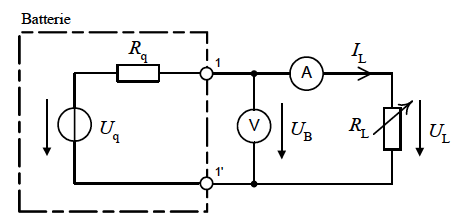
\includegraphics[scale=1]{../img/III/IIIg}
\subsubsection{Messresultate}
Tabellieren Sie die Messwerte und zeichnen Sie die Kennlinie in ein Diagramm $U_B = f(I_L)$. Tabellieren Sie auch die Widerstandswerte.
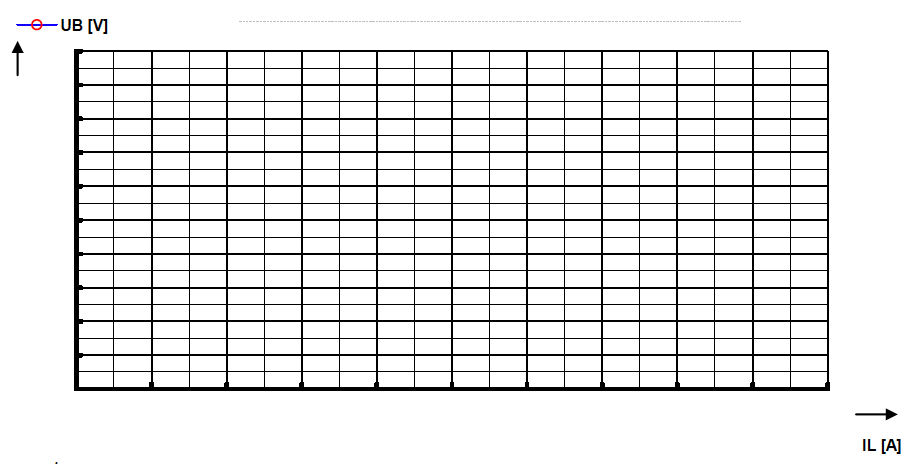
\includegraphics[scale=0.5]{../img/III/IIIh}
\\
\textbf{Messwert:}\\
\begin{tabular}{|c|c|c|c|c|c|c|c|c|c|c|}\hline
$I_L/\text{A}$&&&&&&&&&&\\\hline
$U_B/\text{V}$&&&&&&&&&&\\\hline
$R_L/\Omega$&&&&&&&&&&\\\hline
\end{tabular}
\\\\
Zeichnen Sie zwei Widerstandsgeraden in das Diagramm. Stimmen die Arbeitspunkte überein?
\begin{enumerate}[$a)$]
\item Berechnen Sie den Quellenwiderstand der Batterie. Von welchen Parametern wird dieser abhängig sein?
\item Wie gross ist die Leerlaufspannung, wie gross der Kurzschlussstrom (Berechnung)?
\item Messen Sie den Kurzschlussstrom.
\end{enumerate}